\section{Results}
    \begin{figure*}[ht]
        \centering
        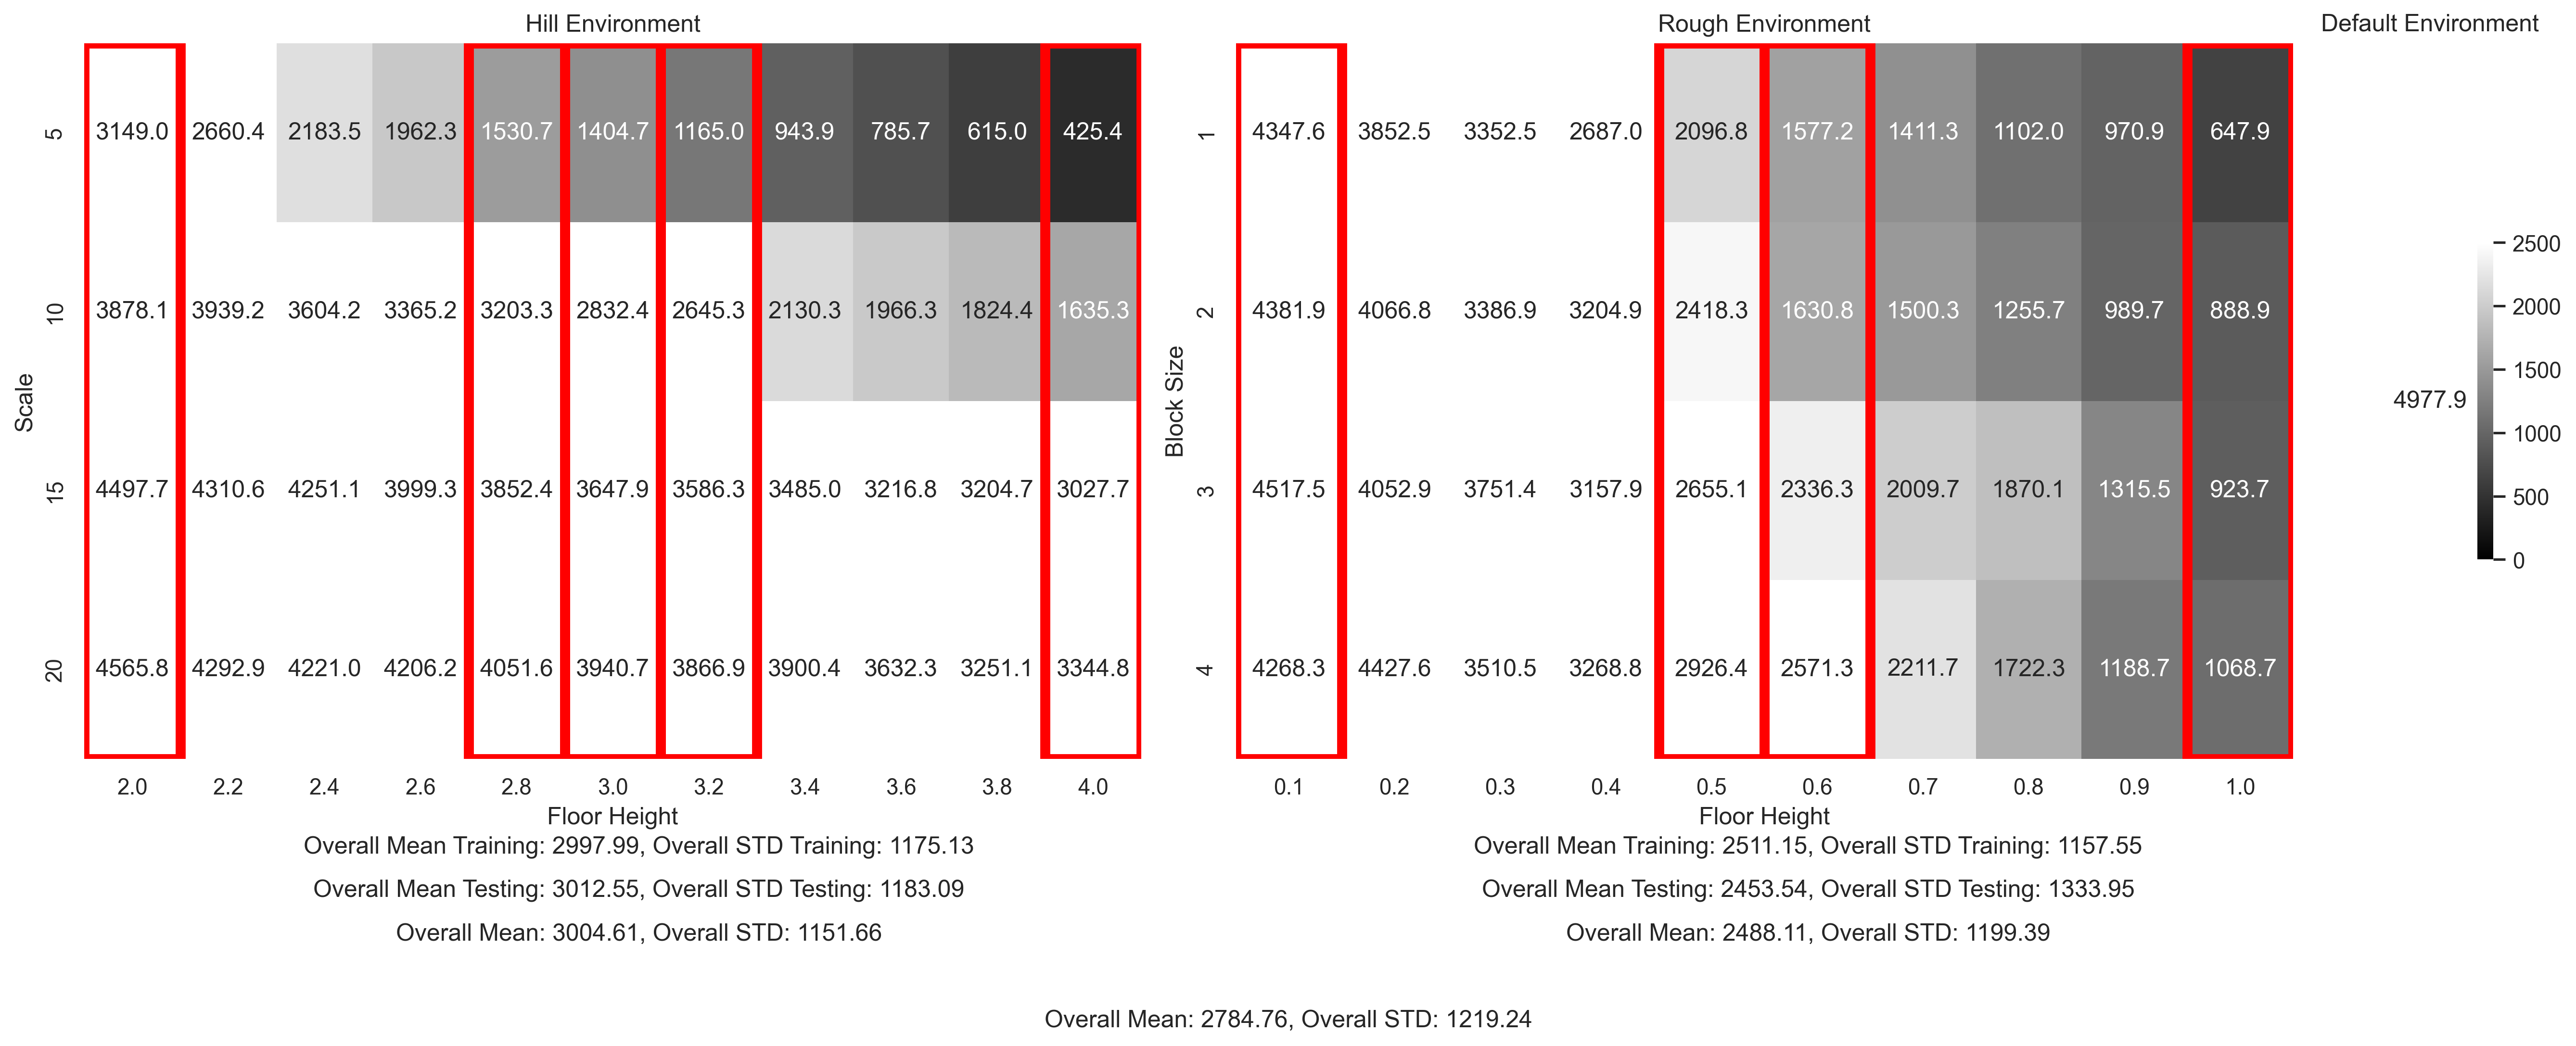
\includegraphics[width=\linewidth]{./resources/generalist_4_2784/fitness_heatmap.png}
        \caption{Fitness heatmap from generalist MC-pair evolved over 5000 generations with partitions disabled}
        \label{fig:fit_heat_5000}
    \end{figure*}

    Figure~\ref{fig:fit_heat_5000} shows the obtained fitness scores for each environment, represented in a heatmap.  The by red enclosed cells indicates the environments from the testing set used for extrapolation testing, while the non-red-enclosed cells represent the environments from the training set used for interpolation testing. 
    
    For the hill environment, the heatmap shows high performance in the environments at the lower left and relatively lower performance when nearing the the upper right. This may indicate inherint complexity in certain environments compared to others. The fitness scores and their standard deviations on the training and testing sets are similar. The training set has a mean fitness score of 2997.99 with a standard deviation of 1175.13, and the testing set has a mean fitness score of 3012.55 with a standard deviation of 1183.09. 
    
    For rough terrain environment, the heatmap also shows high performance in the environments at the lower left and relatively lower performance when nearing the upper right, but also more at the lower right part. The fitness scores and their standard deviations on the training and testing sets are also similar. The training set has a mean fitness score of 2511.15 with a standard deviation of 1157.55, and the testing set has a mean fitness score of 2453.54 with a standard deviation of 1333.95.


    % Figure~\ref{fig:fit_boxplot_5000} shows a boxplot of the fitness distribution.
    % \begin{figure}[ht]
    %     \centering
    %     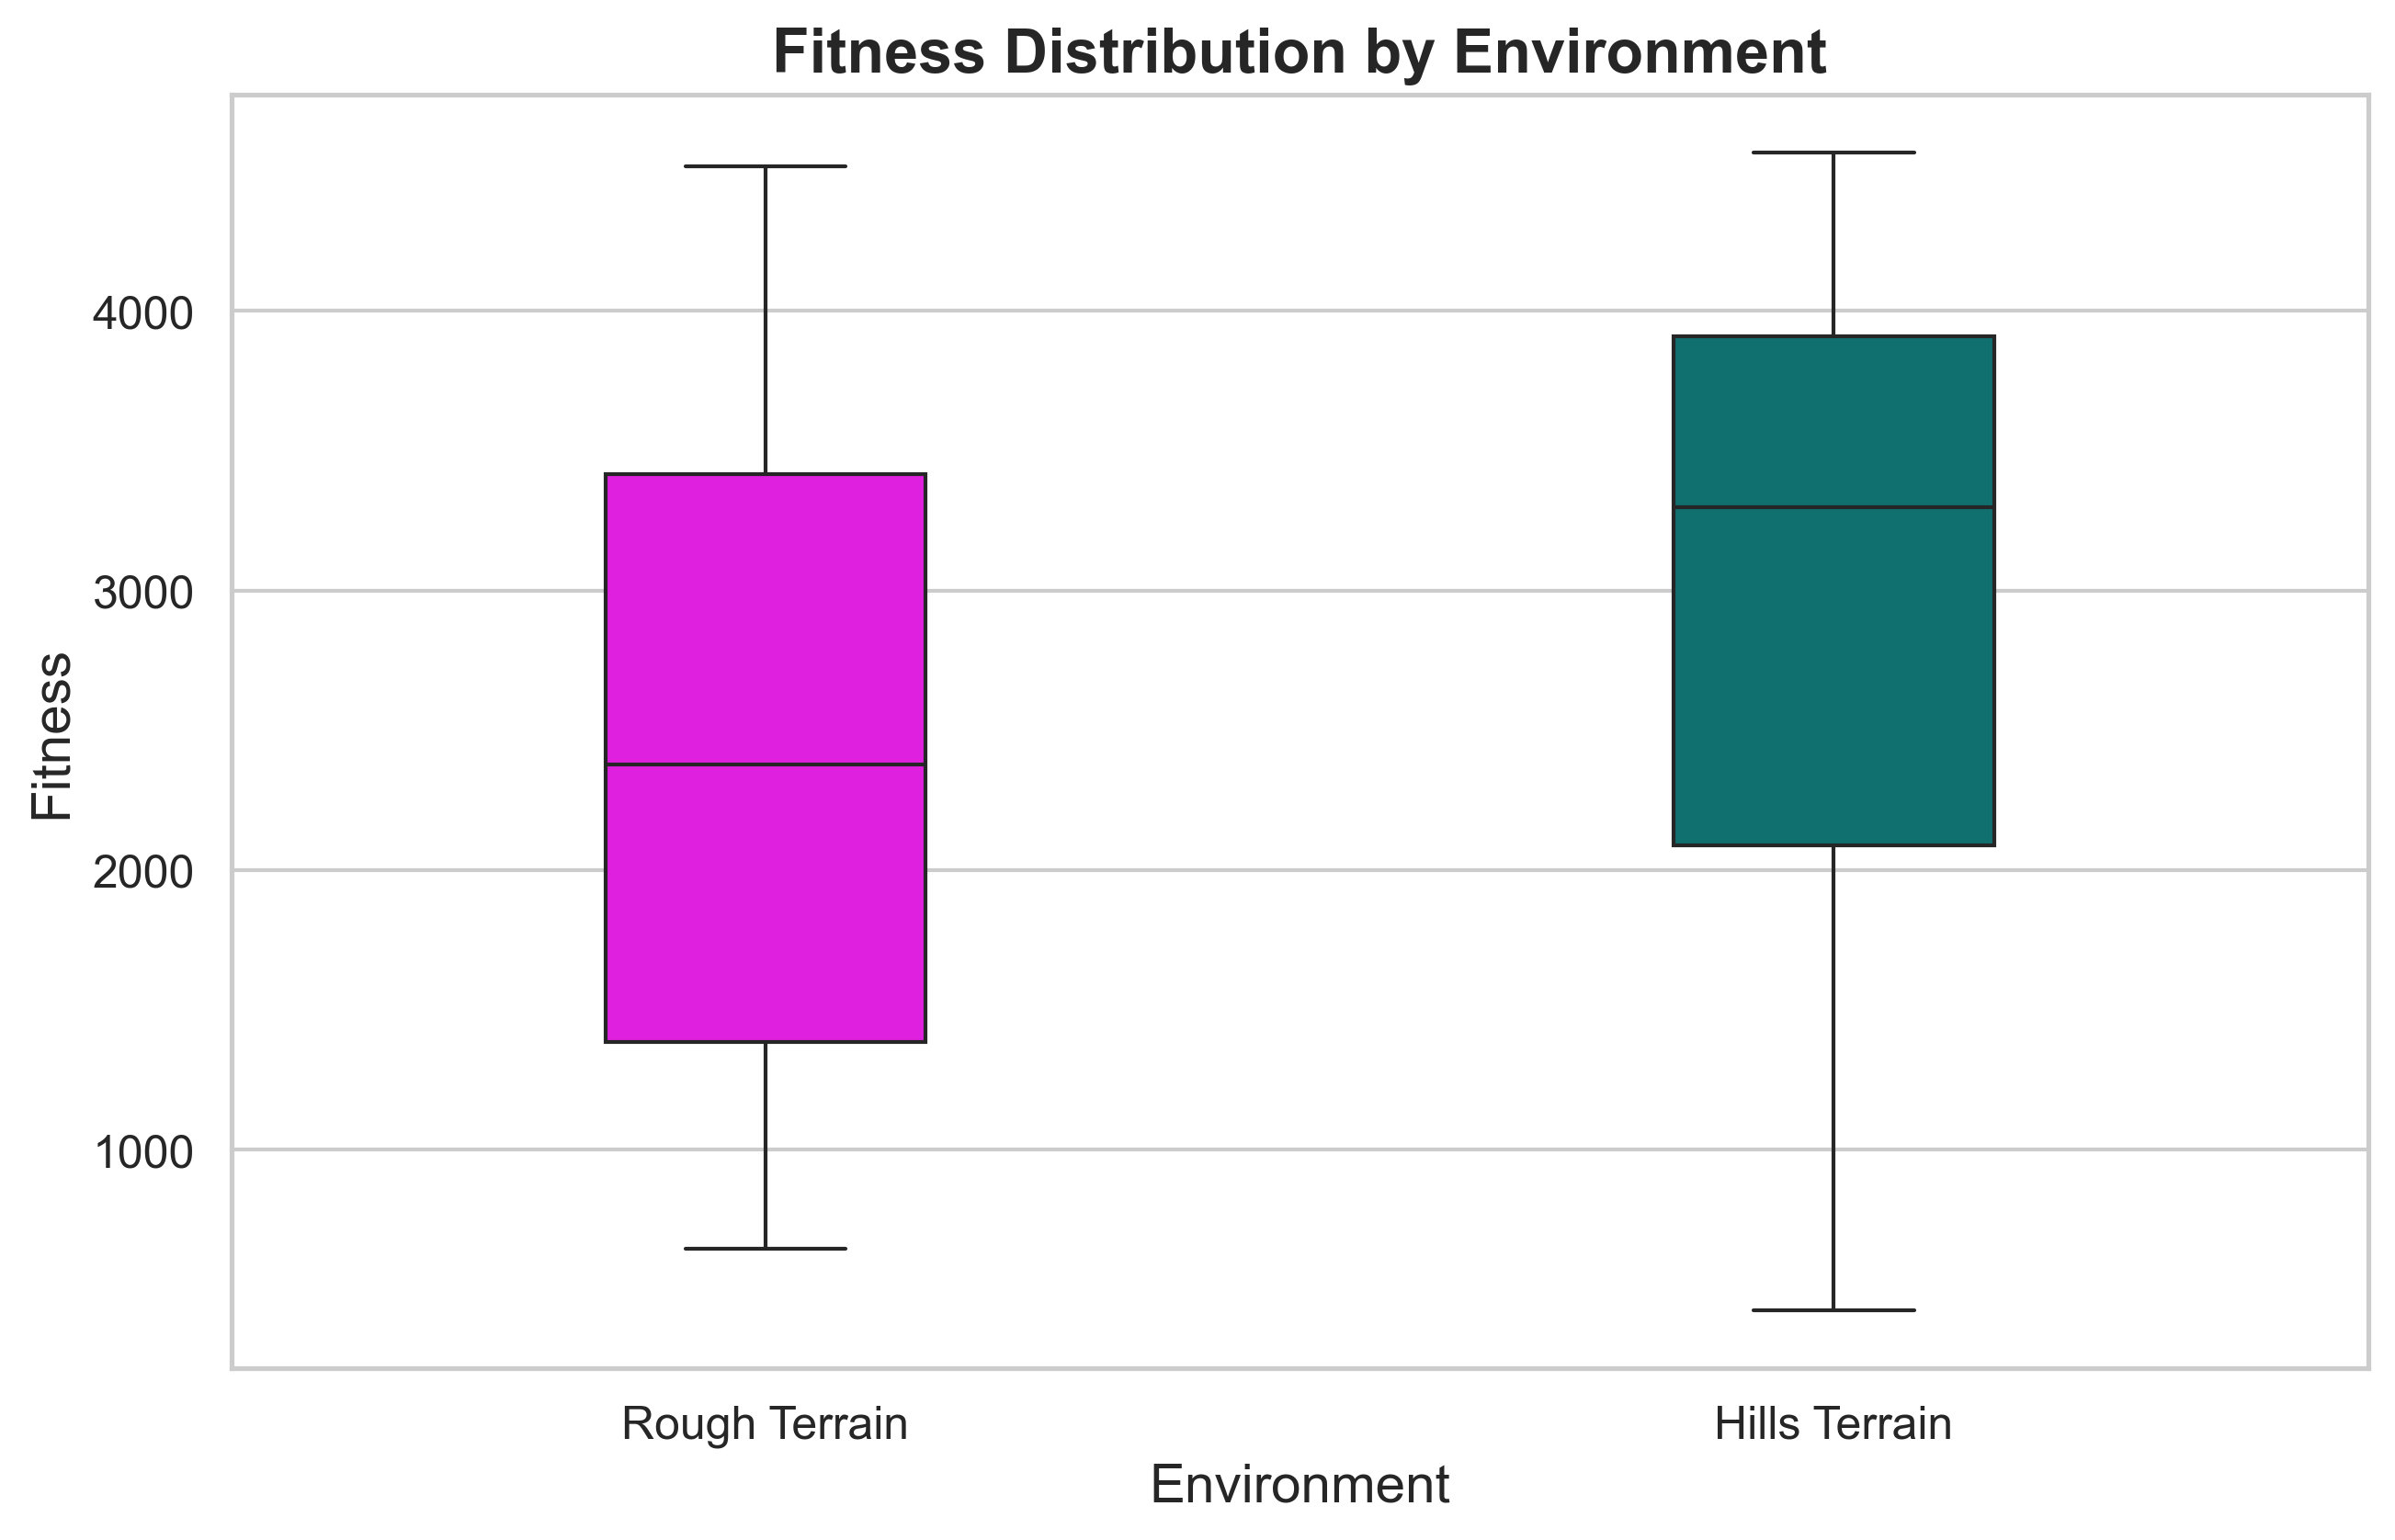
\includegraphics[width=\linewidth]{./resources/generalist_4_2784/fitness_boxplot.png}
    %     \caption{Fitness boxplot}
    %     \label{fig:fit_boxplot_5000}
    % \end{figure}